\documentclass[10pt]{beamer}
\usetheme[
%%% option passed to the outer theme
%    progressstyle=fixedCircCnt,   % fixedCircCnt, movingCircCnt (moving is deault)
  ]{Feather}
  
% If you want to change the colors of the various elements in the theme, edit and uncomment the following lines

% Change the bar colors:
%\setbeamercolor{Feather}{fg=red!20,bg=red}

% Change the color of the structural elements:
%\setbeamercolor{structure}{fg=red}

% Change the frame title text color:
%\setbeamercolor{frametitle}{fg=blue}

% Change the normal text color background:
%\setbeamercolor{normal text}{fg=black,bg=gray!10}

%-------------------------------------------------------
% INCLUDE PACKAGES
%-------------------------------------------------------
%\usepackage{xepersian}
%\settextfont[Scale=1]{IRNazanin}

\usepackage[utf8]{inputenc}
\usepackage[english]{babel}
\usepackage[T1]{fontenc}
\usepackage{helvet}
\usepackage{textpos}


\usepackage{tipa}
\usepackage{listings}
\lstset{language=C++,
	basicstyle=\ttfamily,
	tabsize=4, % tab space width
	showstringspaces=false, % don't mark spaces in strings
	keywordstyle=\color{blue}\ttfamily,
	stringstyle=\color{red}\ttfamily,
	commentstyle=\color{green}\ttfamily,
	morecomment=[l][\color{magenta}]{\#}
}

%-------------------------------------------------------
% DEFFINING AND REDEFINING COMMANDS
%-------------------------------------------------------

% colored hyperlinks
\newcommand{\chref}[2]{
  \href{#1}{{\usebeamercolor[bg]{Feather}#2}}
}

%-------------------------------------------------------
% INFORMATION IN THE TITLE PAGE
%-------------------------------------------------------

\title[] % [] is optional - is placed on the bottom of the sidebar on every slide
{ % is placed on the title page
      \textbf{Fillers\\}
}

\subtitle[Fillers]
{
      \textbf{in programing}
}

\author[S. Zarrin pour]
{      S. Zarrin pour \\
      {
      	\ttfamily sa.zarrinpour@iasbs.ac.ir\\
      	samim56b@gmail.com
  	  }
}

% logo of my university

\institute[]
{
	
      Mathematics Department, Institute for Advance Studies in Basic Sciences\\
      
      
  
  %there must be an empty line above this line - otherwise some unwanted space is added between the university and the country (I do not know why;( )
}

\date{\today \\ \vspace*{0.25cm}\hspace*{0cm}
\includegraphics[height=.5cm]{Feathergraphics/IASBSLOGO.png}}

%-------------------------------------------------------
% THE BODY OF THE PRESENTATION
%-------------------------------------------------------

\begin{document}

%-------------------------------------------------------
% THE TITLEPAGE
%-------------------------------------------------------

{\1% % this is the name of the PDF file for the background
\begin{frame}[plain,noframenumbering] % the plain option removes the header from the title page, noframenumbering removes the numbering of this frame only
  \titlepage % call the title page information from above
\end{frame}}

\addtobeamertemplate{frametitle}{}{%
	\begin{textblock*}{100mm}(.85\textwidth,6.5cm)
		
\includegraphics[height=.75cm,width=2.5cm]{Feathergraphics/IASBSLOGO.png}
\end{textblock*}}

\begin{frame}{Outline}{}
\tableofcontents
\end{frame}

%-------------------------------------------------------
\section{Introduction}
%-------------------------------------------------------
\subsection{Meaning}
\begin{frame}{Introduction}{meaning} 
%-------------------------------------------------------
    \begin{block}{}
		structure
		\begin{itemize}
			\item  {\tt \begin{IPA}/"fIl@/\end{IPA}}
			\item  {\tt noun}
		\end{itemize}
		meaning
		\begin{itemize}
			\item {\tt a thing put in a space or container to fill it.}
			\item {\tt a person or thing that fills a space or container.}
		\end{itemize}
	\end{block}
	\end{frame}
\subsection{Types}
\begin{frame}{Introduction}{filler types} 
%-------------------------------------------------------

	\begin{itemize}
		\item<1- > Bad
		\item<2- > Good
	\end{itemize}

\end{frame}

\section{programming fillers}
\subsection{Introduction}
\begin{frame}{programming fillers}{most used programming fillers} 
%-------------------------------------------------------

	\begin{itemize}
		\item<1- > hello world!
		\item<2- > foo bar
		\item<3- > lorem ipsum
	\end{itemize}

\end{frame}

\subsection{Hello Wolrd!}
\begin{frame}{programming fillers}{Hello World!} 
%-------------------------------------------------------
	novice Usage
	\begin{itemize}
		\item outputs or displays the message "Hello, World!"
		\item very simple in most programming languages
		\item used to illustrate the basic syntax
		\item the first program people write
	\end{itemize}

\end{frame}

\begin{frame}{programming fillers}{Hello World!} 
%-------------------------------------------------------
	Pro Usage
	\begin{itemize}
		\item to introduce novice programmers to a programming language.
		\item Sanity test 
		\item Illustrate a complex notion
	\end{itemize}

\end{frame}

\begin{frame}[fragile]{programming fillers}{Hello World!} 
%-------------------------------------------------------

\begin{block}{Most Known Example : C++}
\begin{lstlisting}
#include <stdio.h>
main() {
    printf("hello, world\n");
}
\end{lstlisting}
\end{block}

\end{frame}
\begin{frame}[fragile]{programming fillers}{Hello World!} 
%-------------------------------------------------------
\begin{block}{The First Used Example (1972): B}
\begin{lstlisting}
main(){
    extrn a,b,c;
    putchar(a);
    putchar(b);
    putchar(c);
    putchar('!*n');
}

a 'hell';
b 'o, w';
c 'orld';
\end{lstlisting}
\end{block}

\end{frame}

\subsection{Foo Bar}
\begin{frame}{programming fillers}{foo bar} 
%-------------------------------------------------------
\begin{itemize}
	\item The etymology of foo is obscure
	\item bar is generally traced to the World War II military slang FUBAR
	\item foo first appeared in 1930 in the comic "Smokey Stover"
	\item placeholder names (metasyntactic variables)
\end{itemize}

\end{frame}

\begin{frame}[fragile]{programming fillers}{foo bar} 
%-------------------------------------------------------
\begin{block}{foo bar as metasyntactic variables : C++}
\begin{lstlisting}
#include <stdio.h>

int main() {
    const char *foo = "Hello";
    const char *bar = "World!";
    fprintf(stdout, "%s %s\n", foo, bar);

    return 0;
}
\end{lstlisting}
\end{block}

\end{frame}

\subsection{Lorem Ipsum}
\begin{frame}{programming fillers}{Lorem Ipsum} 
%-------------------------------------------------------
\begin{itemize}
	\item pseudo-Latin text
	\item placeholder text
	\item demonstrate the visual form of a document without relying on meaningful content (greeking)
	\item design the form of the content before the content has been produced
	\item introduced in the mid-1980s by Aldus Corporation
\end{itemize}

\end{frame}


\begin{frame}{programming fillers}{Lorem Ipsum} 
%-------------------------------------------------------
\begin{figure}[t]
	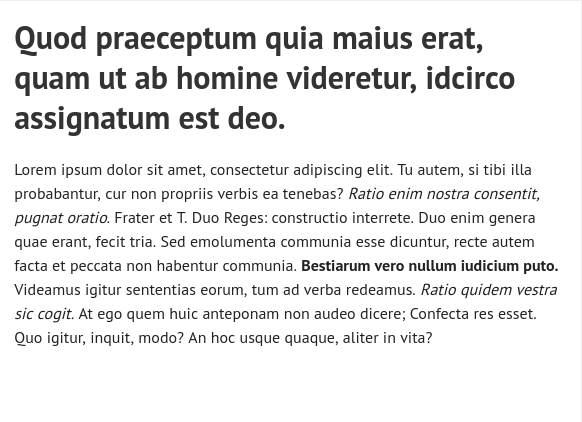
\includegraphics[width=8cm]{Feathergraphics/lorem}
	\centering
\end{figure}
\end{frame}


\section{Q\em\&A}
\begin{frame}{Q\em\&A}{} 
%-------------------------------------------------------
\textbf{"Ask, and it shall be given you!"}\centering\\
\em Matthew 7:7
\end{frame}
\section{References}
\begin{frame}{References}{} 
%-------------------------------------------------------
\begin{itemize}
\item\href{https://www.wikipedia.org/}{https://www.wikipedia.org/}
\item\href{https://loripsum.net/}{https://loripsum.net/}
\end{itemize}
\end{frame}

{\1
\begin{frame}[plain,noframenumbering]
  \finalpage{Thank you for your attention.}
\end{frame}}

\end{document}